% =======================================================================================
%   1. DOCUMENT SETUP & PACKAGES
% =======================================================================================
\documentclass[11pt, a4paper]{article}

% --- ESSENTIAL PACKAGES ---
\usepackage[utf8]{inputenc}
\usepackage[T1]{fontenc}
\usepackage[english]{babel}

% --- PAGE LAYOUT & STYLE ---
\usepackage[a4paper, margin=2.2cm, headheight=15pt, footskip=30pt]{geometry}
\usepackage{graphicx}
\usepackage{float}
\usepackage{caption}
\usepackage{subcaption}
\usepackage{fancyhdr}
\usepackage{xcolor}
\usepackage{titletoc}

% --- TYPOGRAPHY & TEXT ---
\usepackage{lato}
\renewcommand*\familydefault{\sfdefault}
\usepackage{textcomp}
\usepackage{fontawesome5}
\usepackage{microtype} % Improves line breaking and spacing

% Slightly more readable line spacing and allow more flexible breaks
\usepackage{setspace}
\setstretch{1.05}
\sloppy
\emergencystretch=2em

% --- TABLES, LISTS, & BOXES ---
\usepackage{booktabs}
\usepackage{longtable}
\usepackage{tabularx}
\usepackage{array}
\usepackage{enumitem}
\usepackage[skins, breakable, theorems]{tcolorbox}
\tcbuselibrary{skins, breakable, shadows} % Load advanced libraries

% --- TITLES & HYPERLINKS ---
\usepackage{titlesec}
\usepackage{hyperref} % Always load this last

% --- TIKZ FOR DIAGRAMS (STYLIZED WITH CORPORATE PALETTE) ---
\usepackage{tikz}
\usetikzlibrary{shapes, arrows.meta, positioning, shadows, calc, decorations.pathreplacing, backgrounds}
\usepackage{pgfkeys}

% =======================================================================================
%   2. COLOR & STYLE DEFINITIONS
% =======================================================================================

% --- CORPORATE COLOR PALETTE ---
\definecolor{WarlockRed}{HTML}{C11919}
\definecolor{WarlockGold}{HTML}{ECD125}
\definecolor{WarlockDark}{HTML}{1B1818} % Updated to match v5.0 Theme
\definecolor{WarlockGray}{HTML}{333333}
\definecolor{WarlockLightGray}{HTML}{F0F0F0}
\definecolor{WarlockWhite}{HTML}{FFFFFF}

% --- SECTION COLOR PALETTE ---
\definecolor{IntroColor}{HTML}{005A9B}      % Blue
\definecolor{QuickStartColor}{HTML}{00796B} % Green
\definecolor{InstallColor}{HTML}{8E44AD}    % Purple
\definecolor{ModelsColor}{HTML}{D35400}     % Orange
\definecolor{OptimizeColor}{HTML}{27AE60}   % Emerald Green
\definecolor{TroubleColor}{HTML}{C0392B}    % Red
\definecolor{ArchColor}{HTML}{2C3E50}       % Dark Blue
\definecolor{GlossaryColor}{HTML}{7F8C8D}   % Gray
\definecolor{SupportColor}{HTML}{34495E}    % Dark Gray

% --- TEXTBOX COLOR PALETTE ---
\definecolor{InfoFill}{HTML}{E7F3FE}
\definecolor{InfoBorder}{HTML}{005A9B}
\definecolor{WarnFill}{HTML}{FFFBE6}
\definecolor{WarnBorder}{HTML}{FFBE0B}
\definecolor{QuickStartFill}{HTML}{E6FFFA}
\definecolor{QuickStartBorder}{HTML}{00796B}
% New Palette for NEO Engine
\definecolor{NeoFill}{HTML}{F3E5F5}
\definecolor{NeoBorder}{HTML}{8E44AD}

% --- DEFAULT TEXT COLOR APPLICATION ---
\color{WarlockGray}

% =======================================================================================
%   3. DOCUMENT ELEMENT CONFIGURATION
% =======================================================================================

% --- HYPERLINKS ---
\hypersetup{
    colorlinks=true,
    linkcolor=WarlockRed,
    filecolor=WarlockRed,
    urlcolor=WarlockRed,
    pdftitle={Warlock-Studio v5.0 | Technical Documentation and User Manual},
    pdfauthor={Iván Eduardo Chavez Ayub}
}

% --- SECTION & SUBSECTION TITLES ---
\newcommand{\SectionColor}{WarlockGray} % Default color
\newcommand{\setsectioncolor}[1]{\renewcommand{\SectionColor}{#1}}

\titleformat{\section}
  {\normalfont\Large\bfseries}
  {}
  {0em}
  {%
    \begin{tcolorbox}[
        enhanced,
        colback=\SectionColor!90!black,
        colframe=\SectionColor!90!black,
        boxrule=0pt,
        sharp corners,
        halign=center,
        valign=center,
        boxsep=6pt,
        left=0pt, right=0pt, top=0pt, bottom=0pt
    ]
    \color{white}\faBookmark\hspace{0.5em}\thesection.\hspace{1em}#1
    \end{tcolorbox}
  }
\titleformat{\subsection}
  {\normalfont\large\bfseries\color{\SectionColor!80!black}}
  {\faCaretRight\ \thesubsection}
  {1em}
  {}
\titlespacing*{\section}{0pt}{4ex plus 1ex minus .2ex}{3ex plus .2ex}
\titlespacing*{\subsection}{0pt}{2.5ex plus 1ex minus .2ex}{1.3ex plus .2ex}

% --- ENHANCED TEXTBOX DEFINITIONS ---
\newtcolorbox{infobox}[2][]{
    enhanced, breakable,
    colback=InfoFill, colframe=InfoBorder,
    fonttitle=\bfseries, coltitle=InfoBorder,
    title=\faInfoCircle\hspace{0.5em}#2,
    attach boxed title to top left={yshift=-2mm, xshift=3mm},
    boxed title style={colback=InfoBorder, sharp corners},
    coltext=WarlockDark,
    shadow={2mm}{-1mm}{0mm}{black!20!white},
    #1
}
\newtcolorbox{warnbox}[2][]{
    enhanced, breakable,
    colback=WarnFill, colframe=WarnBorder,
    fonttitle=\bfseries, coltitle=WarnBorder!80!black,
    title=\faExclamationTriangle\hspace{0.5em}#2,
    attach boxed title to top left={yshift=-2mm, xshift=3mm},
    boxed title style={colback=WarnBorder, sharp corners},
    coltext=WarlockDark,
    shadow={2mm}{-1mm}{0mm}{black!20!white},
    #1
}
\newtcolorbox{quickstartbox}[2][]{
    enhanced, breakable,
    colback=QuickStartFill, colframe=QuickStartBorder,
    fonttitle=\bfseries, coltitle=QuickStartBorder!80!black,
    title=\faRocket\hspace{0.5em}#2,
    attach boxed title to top left={yshift=-2mm, xshift=3mm},
    boxed title style={colback=QuickStartBorder, sharp corners},
    coltext=WarlockDark,
    shadow={2mm}{-1mm}{0mm}{black!20!white},
    #1
}
% New box for NEO Engine / Hardware features
\newtcolorbox{neobox}[2][]{
    enhanced, breakable,
    colback=NeoFill, colframe=NeoBorder,
    fonttitle=\bfseries, coltitle=NeoBorder!80!black,
    title=\faMicrochip\hspace{0.5em}#2,
    attach boxed title to top left={yshift=-2mm, xshift=3mm},
    boxed title style={colback=NeoBorder, sharp corners},
    coltext=WarlockDark,
    shadow={2mm}{-1mm}{0mm}{black!20!white},
    #1
}

% --- INLINE CODE COMMAND ---
\newcommand{\inlinecode}[1]{\colorbox{WarlockLightGray}{\small\texttt{\detokenize{#1}}}}

% --- HEADER & FOOTER ---
\pagestyle{fancy}
\fancyhf{}
\fancyhead[L]{\textit{Warlock-Studio v5.0}}
\fancyhead[R]{\leftmark}
\fancyfoot[L]{\includegraphics[height=0.8cm]{logo.png}}
\fancyfoot[C]{\thepage}
\fancyfoot[R]{\textcopyright~2025 Warlock-Studio}
\renewcommand{\headrulewidth}{0.4pt}
\renewcommand{\footrulewidth}{0.4pt}
\renewcommand{\sectionmark}[1]{\markboth{\thesection. #1}{}}

% =======================================================================================
%   BEGIN DOCUMENT
% =======================================================================================
\begin{document}

% --- REDESIGNED TITLE PAGE ---
\begin{titlepage}
    \begin{tcolorbox}[
        enhanced, sharp corners,
        colback=WarlockDark, colframe=WarlockGold,
        boxrule=2pt,
        height=\textheight,
        halign=center, valign=center
    ]
        \centering
        \includegraphics[width=0.4\textwidth]{logo.png}\par
        \vfill
        \color{WarlockWhite}
        {\Huge\bfseries\scshape Warlock-Studio\par}
        \vspace{1.5cm}
        \color{WarlockGold}
        \rule{0.6\textwidth}{1pt}\par
        \vspace{0.4cm}
        \color{WarlockWhite}
        {\Large\bfseries Technical Documentation and User Guide\par}
        \vspace{0.2cm}
        {\large Software Version: 5.0 (NEO-Refactor)\par}
        \vspace{0.4cm}
        \color{WarlockGold}
        \rule{0.6\textwidth}{1pt}\par
        \vfill
        {\large Iván Eduardo Chavez Ayub\par}
        \href{https://github.com/Ivan-Ayub97}{\texttt{\color{WarlockGold}\faGithub\ @Ivan-Ayub97}}\par
        \vspace{1.5cm}
        {\large \today\par}
    \end{tcolorbox}
    \thispagestyle{empty}
\end{titlepage}

\newpage
\tableofcontents
\newpage

% =======================================================================================
%   SECTION 1: INTRODUCTION
% =======================================================================================
\setsectioncolor{IntroColor}
\section{Introduction to Warlock-Studio v5.0}
Welcome to Warlock-Studio v5.0 — a major evolutionary leap in AI-powered media enhancement.
This version introduces a robust \textbf{Modular Architecture} and the new \textbf{NEO Engine}, optimizing
stability, hardware diagnostics, and processing efficiency. It provides advanced tools for super-resolution,
artifact removal, and frame generation through an intuitive interface that now includes an \textbf{Integrated Console}
and native \textbf{Drag \& Drop} support.

% =======================================================================================
%   SECTION 2: QUICK START GUIDE
% =======================================================================================
\setsectioncolor{QuickStartColor}
\section{Quick Start Guide}
\begin{quickstartbox}{Accelerated Media Enhancement Procedure}
Follow these steps to process your media using the new v5.0 workflow.
\begin{enumerate}
    \item \textbf{Load Files (Drag \& Drop):} You can now simply \textbf{drag and drop} your image or video files directly onto the application window. Alternatively, click the \textbf{"Select Files"} button.
    \item \textbf{AI Model Selection:} In the \textbf{"AI model"} dropdown menu, select an inference model.
    \begin{itemize}
        \item For photorealistic images, \inlinecode{BSRGANx4} is recommended for texture reconstruction.
        \item For animation/cartoons, \inlinecode{RealESR_Animex4} preserves sharp edges.
        \item For video, \inlinecode{RealESR_Gx4} balances speed and quality.
        \item For increasing framerate, use \inlinecode{RIFE} models (note: Blending controls will hide automatically).
    \end{itemize}
    \item \textbf{Verify Hardware (NEO Engine):} Click the \textbf{Gear Icon} (\faCog) to open Preferences. Check the \textbf{Hardware Diagnostics} to see the "Recommended Tiles" and "Safe VRAM Limit" calculated specifically for your PC.
    \item \textbf{Adjust Settings:} Set the \textbf{"GPU VRAM (GB)"} based on the recommendation. For a quick test, set \textbf{"Input resolution"} to \texttt{75}\%.
    \item \textbf{Start Processing:} Click \textbf{"Make Magic"}. You can now monitor real-time progress and logs via the new \textbf{Integrated Console} at the bottom of the window.
\end{enumerate}
\end{quickstartbox}

% =======================================================================================
%   SECTION 3: INSTALLATION & ARCHITECTURE
% =======================================================================================
\setsectioncolor{InstallColor}
\section{Installation and Modular Architecture}
\subsection{\faDownload\ Installation Process \& Path Change}
Warlock-Studio uses a self-contained offline installer.

\begin{warnbox}{Critical: Installation Directory Change}
In version 5.0, the default installation directory has been migrated from \texttt{Program Files} to:
\begin{center}
\inlinecode{\%userprofile\%\\Documents\\Warlock-Studio}
\end{center}
\textbf{Reason:} This change prevents "Permission Denied" errors on Windows systems with strict UAC. It ensures the application has full read/write access to generate the \inlinecode{warlock_config.json}, write real-time logs, and manage video checkpoints without requiring constant Administrator privileges.
\end{warnbox}

\begin{enumerate}[leftmargin=*]
    \item \textbf{Obtaining the Executable:} Download the `Warlock-Studio-Setup.exe` (Full Installer) from the official repositories.
    \item \textbf{Run the Installer:} Run the setup. It will automatically default to your Documents folder.
    \item \textbf{Launch:} Open Warlock-Studio via the Desktop shortcut.
\end{enumerate}

\subsection{\faMicrochip\ System Requirements}
\begin{table}[H]
    \centering
    \begin{tabularx}{\textwidth}{lX}
        \toprule
        \textbf{Component} & \textbf{Technical Specification} \\
        \midrule
        Operating System & Windows 11 or Windows 10 (64-bit architecture required). \\
        RAM & 8 GB (minimum), 16 GB (recommended). \\
        Graphics Card (GPU) & \textbf{Mandatory Requirement:} GPU with \textbf{DirectX 12} support. \\
        & \textbf{NVIDIA:} CUDA support (Maxwell or newer). \\
        & \textbf{AMD/Intel:} DirectML support. \\
        & \textbf{4+ GB of VRAM} is recommended. \\
        Storage & 2 GB of free disk space. SSD strongly recommended for video I/O. \\
        \bottomrule
    \end{tabularx}
    \caption{Requirements for v5.0. The NEO Engine will verify these upon launch.}
\end{table}

\subsection{\faPuzzlePiece\ Modular File Architecture (v5.0)}
\begin{infobox}{From Monolithic to Modular}
Version 5.0 abandons the single-script structure. The application is now composed of specialized modules to improve stability and maintainability.
\end{infobox}

\begin{itemize}[leftmargin=*]
    \item \textbf{\inlinecode{Warlock-Studio.py} (Core Orchestrator):}
    Manages the main GUI event loop and spawns multiprocessing tasks for AI inference.
    \item \textbf{\inlinecode{warlock_preferences.py} (State Manager):}
    Houses the \textbf{NEO Engine} for hardware telemetry, the \inlinecode{ConfigManager} for JSON persistence, and the OTA Update Manager.
    \item \textbf{\inlinecode{console.py} (I/O Manager):}
    Controls the new \textbf{Integrated Console}, redirecting \texttt{stdout} and \texttt{stderr} streams to the GUI for real-time debugging.
    \item \textbf{\inlinecode{drag_drop.py} (Event Wrapper):}
    Implements the \inlinecode{DnDCTk} class to handle native OS Drag \& Drop events.
    \item \textbf{Assets:}
    Includes \inlinecode{ffmpeg.exe}, \inlinecode{exiftool.exe}, and the AI Models (`.onnx`) in the \texttt{AI-onnx} directory.
\end{itemize}


% =======================================================================================
%   SECTION 4: DETAILED AI MODEL GUIDE
% =======================================================================================
\setsectioncolor{ModelsColor}
\section{Detailed Analysis of Inference Models}

\begin{infobox}{Dynamic Interface Adaptation}
In v5.0, the interface adapts to your model selection. Selecting a \textbf{RIFE} model will automatically hide "Blending" controls and reveal "Frame Generation" options. Selecting an \textbf{Upscaling} model does the reverse.
\end{infobox}

\subsection{\faTable\ Model Comparison Matrix}
\begin{longtable}{p{2.8cm} p{1.8cm} p{1.2cm} p{1.5cm} p{7.2cm}}
\toprule
\textbf{Model} & \textbf{Function} & \textbf{Scale} & \textbf{VRAM} & \textbf{Use Case} \\
\midrule
\endhead
\multicolumn{5}{c}{\textit{\textbf{\faEraser\ Denoising}}} \\
\midrule
\texttt{IRCNN\_Mx1} & Denoise & x1 & 4.0 & Moderate noise reduction (JPEG artifacts). \\
\texttt{IRCNN\_Lx1} & Denoise & x1 & 4.0 & Intensive noise reduction for degraded images. \\
\midrule
\multicolumn{5}{c}{\textit{\textbf{\faTachometerAlt\ High-Fidelity Upscaling}}} \\
\midrule
\texttt{BSRGANx4} & Upscale & x4 & 0.6 & Photorealistic texture synthesis. Best for portraits/nature. \\
\texttt{RealESRGANx4} & Upscale & x4 & 0.6 & General-purpose robust reconstruction. \\
\midrule
\multicolumn{5}{c}{\textit{\textbf{\faBolt\ High-Speed Upscaling}}} \\
\midrule
\texttt{RealESR\_Gx4} & Upscale & x4 & 2.2 & Fastest model. Optimized for video. \\
\texttt{RealESR\_Animex4} & Upscale & x4 & 2.2 & Optimized for Anime/Cartoons (clean lines). \\
\midrule
\multicolumn{5}{c}{\textit{\textbf{\faUserCircle\ Facial Restoration}}} \\
\midrule
\texttt{GFPGAN} & Restore & x1 & 1.8 & Face reconstruction. v5.0 enforces \textbf{Float32} precision for stability. \\
\midrule
\multicolumn{5}{c}{\textit{\textbf{\faFilm\ Frame Interpolation (FluidFrames)}}} \\
\midrule
\texttt{RIFE} & Interpolate & N/A & \textasciitilde{}1.5 & Generates intermediate frames (x2, x4, x8). \\
\texttt{RIFE\_Lite} & Interpolate & N/A & \textasciitilde{}1.2 & Faster variant for lower-end GPUs. \\
\midrule
\bottomrule
\caption{Technical guide for AI models. VRAM values are base estimates.}
\label{tab:modelos}
\end{longtable}

% =======================================================================================
%   SECTION 5: OPTIMIZATION & NEO ENGINE
% =======================================================================================
\setsectioncolor{OptimizeColor}
\section{Performance Optimization and NEO Engine}

\subsection{\faMagic\ The NEO Engine}
\begin{neobox}{Automatic Hardware Heuristics}
Warlock-Studio v5.0 introduces the \textbf{NEO Engine} (located in \inlinecode{warlock_preferences.py}). This system scans your CPU, RAM, and GPU capabilities in real-time to generate \textbf{Smart Recommendations}.
\end{neobox}

\begin{itemize}[leftmargin=*, itemsep=2pt]
    \item \textbf{Safe VRAM Limit:} The engine calculates a safe buffer using the formula: $\max(0.5, \text{Physical VRAM} - 1.5 \text{ GB})$.
    \item \textbf{Recommended Tiles:} It suggests the optimal \inlinecode{tiles_resolution} to maximize speed while preventing Out-Of-Memory (OOM) crashes.
    \item \textbf{Thread Concurrency:} It analyzes your CPU topology (physical vs. logical cores) to suggest safe multithreading levels for video processing.
\end{itemize}

\subsection{\faSlidersH\ Critical Parameters}
\begin{itemize}[leftmargin=*, itemsep=2pt]
    \item \textbf{Input Resolution \%:} Setting this to \textbf{75\%} drastically reduces load with minimal quality loss.
    \item \textbf{AI Multithreading:} (Video only) Processes multiple frames in parallel. Use the NEO Engine's recommendation to avoid system freezing.
    \item \textbf{Keep Frames:} Enable this (\inlinecode{selected_keep_frames = True}) if you plan to experiment with different video encoding codecs later.
\end{itemize}

% =======================================================================================
%   SECTION 6: TROUBLESHOOTING
% =======================================================================================
\setsectioncolor{TroubleColor}
\section{Diagnostics and Troubleshooting}
\begin{warnbox}{Integrated Console}
Use the new **Integrated Console** at the bottom of the app window to view real-time error logs, warnings, and processing status. You can search, copy, and save these logs.
\end{warnbox}

\begin{description}[leftmargin=*, style=nextline, itemsep=0.8em]
    \item[\faBan\ Error: "FFmpeg encoding failed..." / Fallback Active]
        \textbf{Diagnosis:} The selected hardware codec (e.g., \inlinecode{hevc_nvenc}) failed due to driver issues or resource locking.
        \textbf{v5.0 Solution:} The system now features an \textbf{Automatic Fallback}. If the GPU encoder fails, it automatically switches to the CPU-based \inlinecode{libx264} encoder to ensure the video is finished. Check the console for yellow warnings indicating this switch.

    \item[\faMemory\ Error: "Out of memory" / OOM Recovery]
        \textbf{Diagnosis:} VRAM exhaustion during tiling.
        \textbf{v5.0 Solution:} The application detects this exception and triggers \textbf{Recursive Dynamic Tiling}. It automatically halves the tile resolution (e.g., 100\% $\to$ 50\%) and retries the frame. You do not need to restart the process manually.

    \item[\faRocket\ Error: "Failed to load model" (ONNX)]
        \textbf{Diagnosis:} Issue initializing the execution provider.
        \textbf{Solution:} v5.0 implements a strict priority chain: CUDA $\to$ DirectML $\to$ CPU. Ensure your GPU drivers are up to date. If using an older NVIDIA card, the system may default to DirectML or CPU.

    \item[\faTachometerAlt\ Error: "NaN" (Not a Number)]
        \textbf{Diagnosis:} GPU Driver Timeout (TDR).
        \textbf{Solution:} Restart the process without deleting the temp frames folder. The app will resume from the last successful frame.
\end{description}

% =======================================================================================
%   SECTION 7: ADVANCED TECHNICAL ARCHITECTURE
% =======================================================================================
\setsectioncolor{ArchColor}
\section{Software Architecture Analysis (v5.0)}

\subsection{\faCogs\ Modular Inference Engine}
Warlock-Studio v5.0 utilizes a robust \textbf{ONNX Runtime} backend managed by the \inlinecode{create_onnx_session} factory in the core orchestrator. It enforces strict integer typing for device IDs to ensure compatibility with rigid DirectML backends.

\subsection{\faSyncAlt\ Lossless Intermediate Pipeline}
In v5.0, the video extraction pipeline (\inlinecode{extract_video_frames}) strictly enforces the use of \textbf{.PNG} containers for temporary frames. This eliminates the generation loss previously caused by JPEG artifacts before the image entered the neural network.

\subsection{\faThLarge\ Architecture Diagram (Modular)}
\noindent
Updated component-level architecture illustrating the new modular design and the interaction between the GUI, the NEO Engine, and the Core Orchestrator.

\begin{figure}[H]
    \centering
    \resizebox{\textwidth}{!}{%
    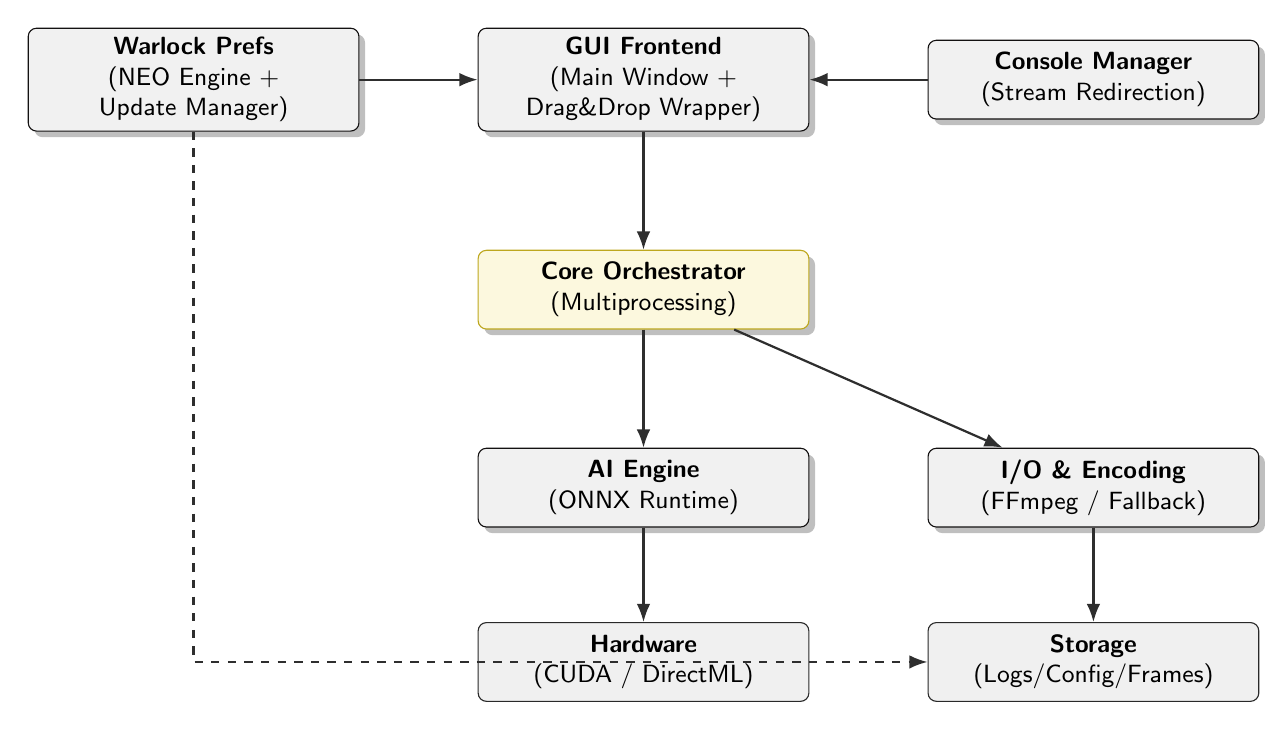
\begin{tikzpicture}[node distance=12mm, every node/.style={font=\small}]
      \tikzset{
        module/.style={rectangle, rounded corners=3pt, draw=WarlockDark!70!black, fill=WarlockDark!6, minimum width=42mm, minimum height=10mm, align=center, drop shadow},
        core/.style={rectangle, rounded corners=3pt, draw=WarlockGold!80!black, fill=WarlockGold!15, minimum width=42mm, minimum height=10mm, align=center, drop shadow},
        hw/.style={rectangle, rounded corners=3pt, draw=WarlockGray!80!black, fill=WarlockLightGray, minimum width=42mm, minimum height=10mm, align=center},
        line/.style={-Latex, thick, color=WarlockGray!90!black}
      }

      % Nodes
      \node[module] (gui) {\textbf{GUI Frontend}\\(Main Window +\\Drag\&Drop Wrapper)};
      \node[module, left=15mm of gui] (prefs) {\textbf{Warlock Prefs}\\(NEO Engine +\\Update Manager)};
      \node[module, right=15mm of gui] (console) {\textbf{Console Manager}\\(Stream Redirection)};

      \node[core, below=15mm of gui] (orch) {\textbf{Core Orchestrator}\\(Multiprocessing)};

      \node[module, below=15mm of orch] (ai) {\textbf{AI Engine}\\(ONNX Runtime)};
      \node[module, right=15mm of ai] (io) {\textbf{I/O \& Encoding}\\(FFmpeg / Fallback)};

      \node[hw, below=12mm of ai] (gpu) {\textbf{Hardware}\\(CUDA / DirectML)};
      \node[hw, below=12mm of io] (disk) {\textbf{Storage}\\(Logs/Config/Frames)};

      % Connections
      \draw[line] (prefs) -- (gui);
      \draw[line] (console) -- (gui);
      \draw[line] (gui) -- (orch);
      \draw[line] (orch) -- (ai);
      \draw[line] (orch) -- (io);
      \draw[line] (ai) -- (gpu);
      \draw[line] (io) -- (disk);
      \draw[line, dashed] (prefs) |- (disk);

    \end{tikzpicture}
    }
    \caption{Warlock-Studio v5.0 Modular Component Architecture.}
\end{figure}

% =======================================================================================
%   SECTION 8: GLOSSARY
% =======================================================================================
\setsectioncolor{GlossaryColor}
\section{Glossary}
\begin{description}[leftmargin=*, style=nextline, itemsep=0.8em]
    \item[NEO Engine] The new heuristic subsystem in v5.0 responsible for hardware scanning, diagnostics, and configuration recommendation.
    \item[Modular Architecture] A software design technique that splits the code into separate, independent modules (`console`, `preferences`, `core`) to improve maintainability.
    \item[ONNX Runtime] The cross-platform engine used to run the AI models. v5.0 enforces strict device ID typing.
    \item[OOM Recovery] (Out Of Memory) An automatic mechanism that reduces tile size when VRAM is exhausted to prevent crashes.
    \item[DirectML] (Direct Machine Learning) API used for GPU acceleration on AMD and Intel cards.
\end{description}

% =======================================================================================
%   SECTION 9: SUPPORT & CONTRIBUTIONS
% =======================================================================================
\setsectioncolor{SupportColor}
\section{Support and Community}
\begin{itemize}[leftmargin=*]
    \item \textbf{\faBook\ Manual:} Click the \textbf{Book Icon} in the app header to open this PDF document.
    \item \textbf{\faBug\ Reporting Issues:} Report bugs on GitHub. Please attach the \inlinecode{error_log.txt} file located in your \textbf{Documents} folder.
    \item \textbf{\faSync\ Updates:} Use the internal \textbf{Update Manager} (Gear Icon $\to$ Check Updates) to download the latest version directly.
    \item \textbf{\faEnvelope\ Contact:} For non-bug related inquiries: \href{mailto:negroayub97@gmail.com}{\texttt{negroayub97@gmail.com}}.
\end{itemize}
\vspace{1cm}
\centering
\textbf{Thank you for using Warlock-Studio v5.0.}

% =======================================================================================
%   END OF DOCUMENT
% =======================================================================================
\end{document}
